\section{Results}

All the following benchmarks were conducted on a local machine running Ubuntu
22.04 LTS with a 6-core, 12-thread CPU and 32GB of RAM\@. All tests were
conducted on the OpenJDK VM Corretto 21. The JVM was configured with a minimum
heap size of 1024MB and a maximum heap size of 16GB\@.

For both the Apache Bench and JMeter tests, we simulate a 1000-request warmup
period for each route with a concurrent user load of 32 users. The warmup
period is followed by the actual test period, during which we simulate 256
requests per user, scaling in increments up to 128 concurrent users.

The results are presented in the form of throughput (number of requests per
second) for each template engine, with the x-axis representing the number of
concurrent users and the y-axis representing the throughput in requests per
second.

Both the Quarkus and Spring MVC implementations were configured with an output
buffer size of 8KB, despite the Quarkus implementation not enabling PSSR at
this size. This configuration was chosen to ensure consistency across Spring
MVC and Quarkus, as the Spring MVC implementation does not support PSSR for the
tested templates.

Since the obtained results for JMeter and Apache Bench show no significant
differences, only the JMeter results will be presented.

\subsection{Presentations Results}

The results in Figure~\ref{fig:presentations-webflux-jmeter} depict the
throughput (number of requests per second) for each template engine, with
concurrent users ranging from 1 to 128, from left to right. The benchmarks
include HtmlFlow using suspendable web templates (\textit{HtmlFlow-Susp},
equivalent to the approach shown in Listing~\ref{lst:presentation-flow}),
Jstachio using Virtual Threads with the \texttt{Iterable} interface
(\textit{Jstachio-Virtual}), and Thymeleaf using the reactive View Resolver
driver (Thymeleaf-Rx).
\textit{Blocking} and \textit{Virtual} represent the average throughput of the
blocking approaches (i.e., KotlinX, Rocker, Jstachio, Pebble, Freemarker,
Trimou, HtmlFlow, and Thymeleaf) when run in the context of a separate
coroutine dispatcher or Virtual Threads, respectively.

We show the \textit{HtmlFlow-Susp}, \textit{Jstachio-Virtual}, and \textit{Thymeleaf-Rx} engines
separately to observe the performance of the non-blocking engines when using
the Suspending, Virtual Thread, and Reactive approaches. The \textit{Blocking}
and \textit{Virtual} are aggregated due to the similar performance of different
engines when using those approaches.

\begin{figure}[h]
     \centering
     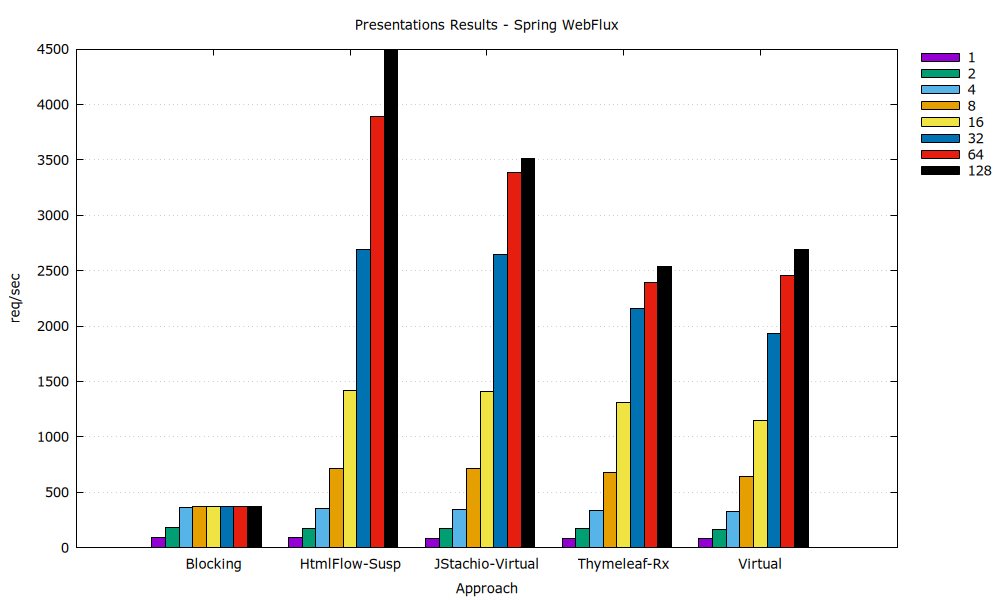
\includegraphics[width=0.8\textwidth]{./Graphs/presentations-webflux-jmeter.png}
     \caption{Presentation Benchmark Results in Spring WebFlux with JMeter}\label{fig:presentations-webflux-jmeter}
\end{figure}

The results show that when using the blocking template engines with a separate
coroutine dispatcher, the engines are unable to scale effectively beyond 16
concurrent users. In contrast, the non-blocking engines scale effectively up to
128 concurrent users, with HtmlFlow achieving approximately 11,000 requests per
second. When using the blocking approaches in the context of Virtual Threads
(achieving non-blocking I/O), the engines scale effectively up to 128
concurrent users, with Jstachio matching HtmlFlow`s performance at
approximately 11,000 requests per second. Thymeleaf, using the reactive View
Resolver driver, also scales to 128 users, albeit less effectively, achieving
around 8,500 requests per second.

\begin{figure}[h]
     \centering
     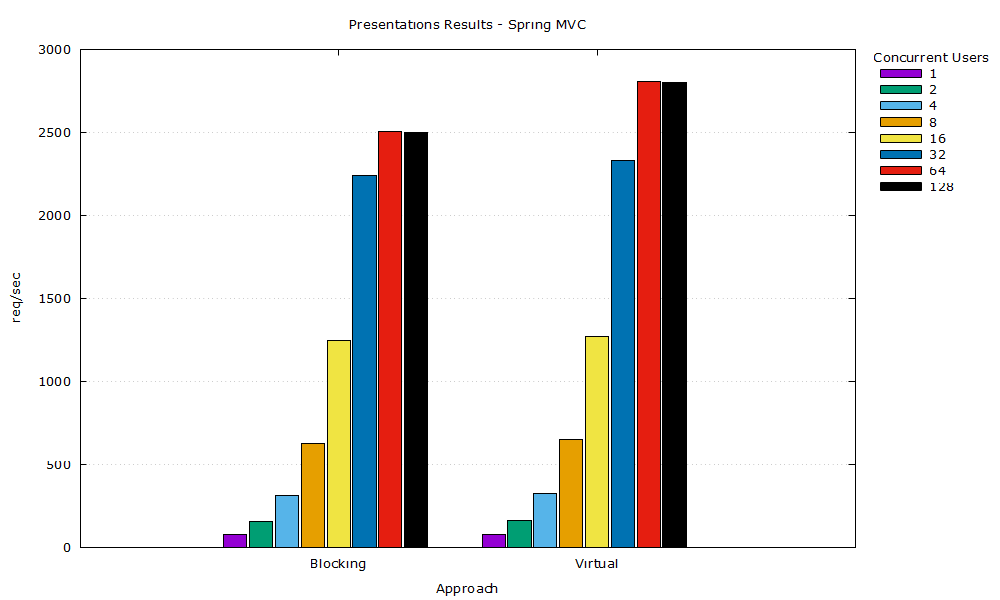
\includegraphics[width=0.8\textwidth]{./Graphs/presentations-springmvc-jmeter.png}
     \caption{Presentation Benchmark Results in Spring MVC with JMeter}\label{fig:presentations-springmvc-jmeter}
\end{figure}

% The results for the Spring MVC implementation, shown in
% Figure~\ref{fig:presentations-springmvc-jmeter}, compare two approaches:
% \textit{Blocking}, which uses platform threads with \texttt{StreamingResponseBody},
% and \textit{Virtual}, which uses Virtual Threads. Both approaches scale
% effectively up to 128 concurrent users, with the Virtual Thread approach
% achieving a slightly higher throughput of 9,000 requests per second. However,
% these values are slightly lower than those observed in the Spring WebFlux
% implementation.

The results for the Spring MVC implementation, shown in
Figure~\ref{fig:presentations-springmvc-jmeter}, compare two synchronous
approaches: \textit{Blocking}, which uses platform threads with
\texttt{StreamingResponseBody}, and \textit{Virtual}, which uses Virtual
Threads. Note that for Spring MVC, which follows a thread-per-request
architecture, neither of the asynchronous approaches—\textbf{Reactive} nor
\textbf{Suspendable}—described in Section~\ref{sec:bench} are applicable. Regarding the
synchronous strategy, both \textit{Blocking} and \textit{Virtual} scale
effectively up to 128 concurrent users, with the Virtual Threads approach
achieving a slightly higher throughput of approximately 9,000 requests per
second. However, these values are slightly lower than those observed in the
Spring WebFlux implementation.

\begin{figure}[h]
     \centering
     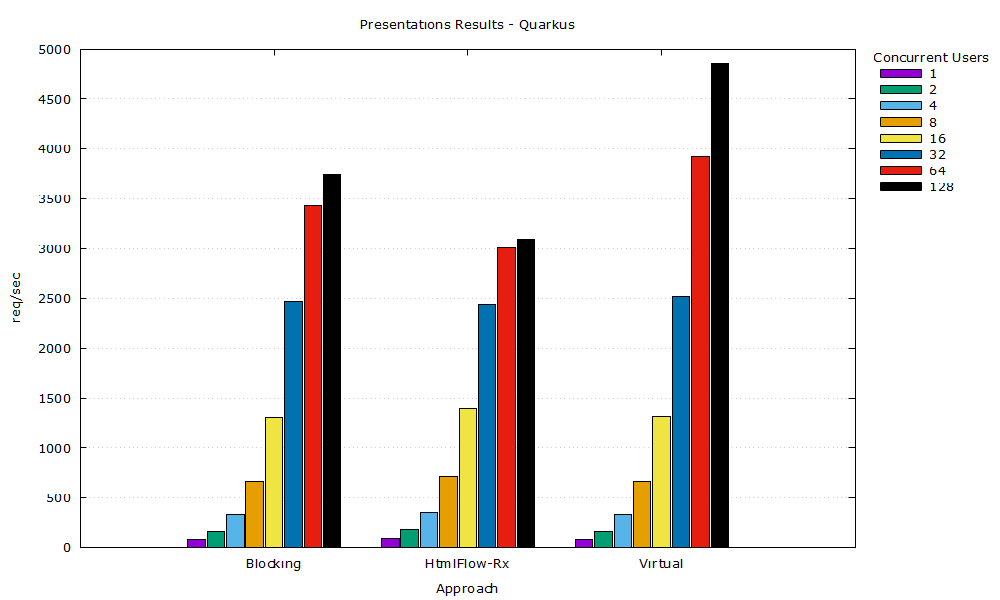
\includegraphics[width=0.8\textwidth]{./Graphs/presentations-quarkus-jmeter.png}
     \caption{Presentation Benchmark Results in Quarkus with JMeter}\label{fig:presentations-quarkus-jmeter}
\end{figure}

The results for the Quarkus implementation, shown in
Figure~\ref{fig:presentations-quarkus-jmeter}, indicate that Quarkus handles
synchronous approaches more efficiently than Spring WebFlux. The blocking
engines scale up to 128 concurrent users, achieving up to 10,000 requests per
second. While the use of Virtual Threads results in a slightly higher
throughput, the difference is negligible, with both approaches delivering
comparable performance.

Additionally, \textit{HtmlFlow-Rx}, a reactive implementation of the HtmlFlow
template engine (equivalent to the approach shown in
Listing~\ref{lst:presentation-observable}) that utilizes Quarkus's reactive
programming model, achieved throughput similar to the \textit{Blocking} and
\textit{Virtual}
approaches—approximately 10,000 requests per second. This demonstrates that
Quarkus's reactive programming model is effective for enabling PSSR\@. However,
there is no significant difference in performance between the reactive and
synchronous approaches, indicating that the reactive model does not provide a
substantial advantage over synchronous approaches in this context.

\subsection{Stocks Results}

\begin{figure}[h]
     \centering
     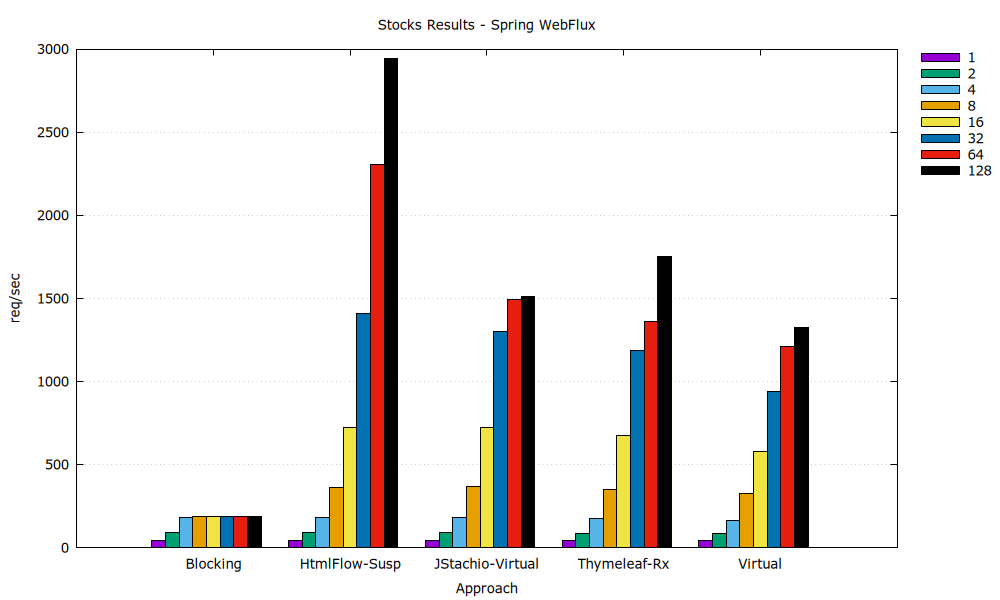
\includegraphics[width=0.8\textwidth]{./Graphs/stocks-webflux-jmeter.png}
     \caption{Stocks Benchmark Results in Spring WebFlux with JMeter}\label{fig:stocks-webflux-jmeter}
\end{figure}

The results in Figure~\ref{fig:stocks-webflux-jmeter} use the same template
engines and approaches as the previous benchmark, but replace the data model
with the more complex Stock class, including 20 instances. Despite the
increased complexity and number of instances, the scalability of the engines
remains largely unaffected. However, throughput is reduced by approximately 50
percent across all engines, with HtmlFlow achieving 6,000 requests per second.
Since the \texttt{Stock} class\ contains more data properties than the
\texttt{Presentation} class, the data binding to the template engine adds
overhead, which explains the reduced performance. The Thymeleaf implementation
using the reactive View Resolver driver reaches 5,000 requests per second,
suggesting that the performance drop compared to the Presentation benchmark is
not substantial.

\begin{figure}[h]
     \centering
     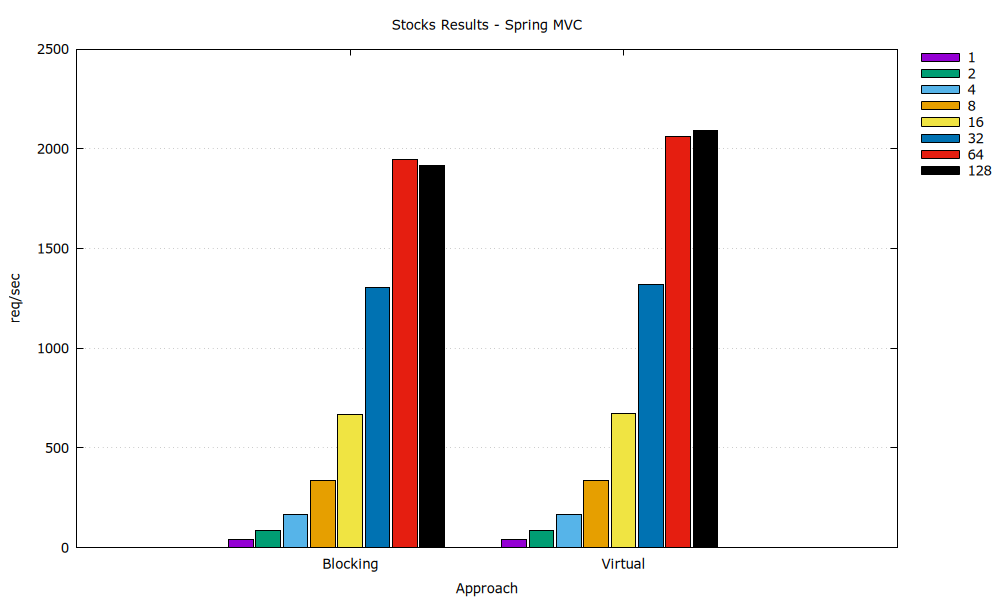
\includegraphics[width=0.8\textwidth]{./Graphs/stocks-springmvc-jmeter.png}
     \caption{Stocks Benchmark Results in Spring MVC with JMeter}\label{fig:stocks-springmvc-jmeter}
\end{figure}

The results observed in Figure~\ref{fig:stocks-springmvc-jmeter} show that the
Spring MVC implementation using the blocking approach with
\texttt{StreamingResponseBody} achieves a throughput of up to 5500 requests per
second, while no significant change is observed when using Virtual Threads. As
such, both approaches scale effectively up to 128 concurrent users.

\begin{figure}[h]
     \centering
     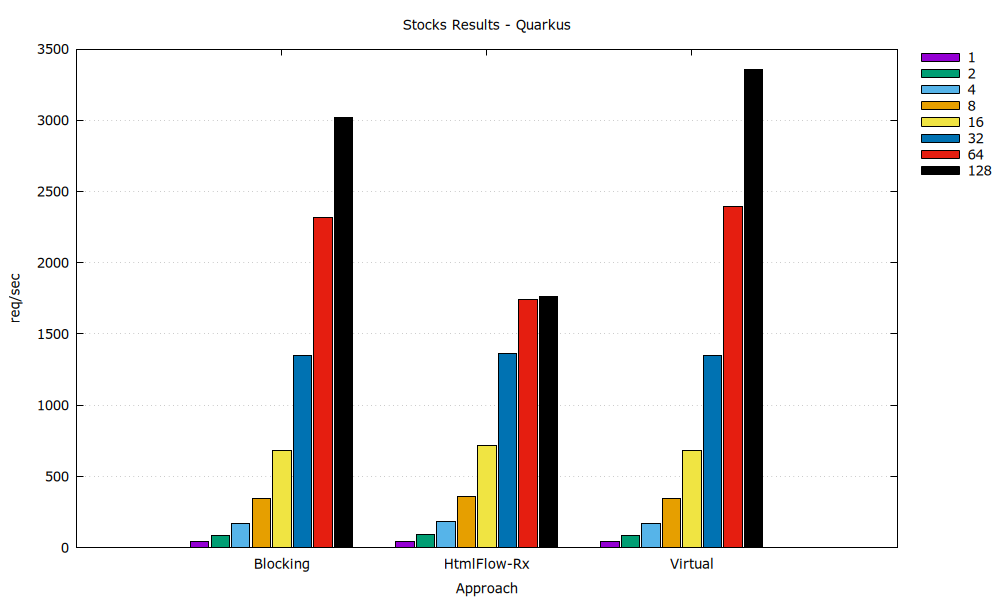
\includegraphics[width=0.8\textwidth]{./Graphs/stocks-quarkus-jmeter.png}
     \caption{Stocks Benchmark Results in Quarkus with JMeter}\label{fig:stocks-quarkus-jmeter}
\end{figure}

The results depicted in Figure~\ref{fig:stocks-quarkus-jmeter} show that the
Quarkus implementation scales effectively up to 128 concurrent users, achieving
performance comparable to the Spring WebFlux implementation. The blocking
engines reach approximately 5,500 requests per second, and once again, there is
no significant difference between the \textit{Blocking} and \textit{Virtual}
approaches, with both achieving similar results.

In addition to the blocking engines, the \textit{HtmlFlow-Rx} approach also
achieves a throughput of approximately 5,500 requests per second, matching the
performance of the \textit{Blocking} and \textit{Virtual} approaches. This
further demonstrates that there is no significant difference in performance
between the reactive and synchronous approaches in this context.

The results of the benchmarks show that non-blocking engines, through the use
of reactive programming, Kotlin coroutines, or Java virtual threads, are able
to scale effectively up to 128 concurrent users. Out of all the tested
frameworks, Spring Webflux showed itself the most effective at enabling PSSR,
mostly due to its native support for Publish and Subscriber interfaces, which
allow for HTML content to be progressively streamed to the client. Quarkus also
enabled PSSR effectively, but it required additional configuration of the
\texttt{OutputBuffer} size to achieve the same results as Spring Webflux. The
Spring MVC implementation, on the other hand, did not enable PSSR for the
tested templates.

Additionally, the results show that approaches using Virtual Threads are able
to scale as effectively as those using reactive programming or Kotlin
coroutines, allowing \textit{external} DSLs to be used in a non-blocking
context, effectively enabling PSSR\@.